\chapter{Análise Bibliográfica sobre a possível relação da tecnologia com depressão, ansiedade e insônia, por Gustavo Macedo de Carvalho\label{chap:bibliometria:GustavoMacCar}}

\section{Planejamento do estudo}
Com o passar do tempo, a tecnologia encontra-se cada vez mais presente em nosso cotidiano. Dispomos de \texttt{smartphones} , \texttt{tablets} , \texttt{smart} \texttt{TVs} , computadores poderosos, \smartwatches\ , dentre outros dispositivos que pareceriam
dignos de ficção científica há cerca de 20 anos atrás, no início da década de 2000. Não há dúvidas que a tecnologia trás muitas vantagens para nossas vidas, como: entretenimento, facilidade de comunicação e aumento da produtividade.
Porém, também podemos apontar algumas desvantagens, como: um certo distanciamento entre as pessoas e o fato de nos tornarmos, de certa forma, dependentes da tecnologia. Entretanto, será que além dessas desvantagens citadas, a tecnologia também
pode estar relacionada com problemas mais sérios, como algumas enfermidades psiquiátricas? Este estudo busca investigar uma possível correlação entre a tecnologia e depressão, ansiedade e insônia.
\begin{itemize}
    \item Como a investigação sobre esse tema ocorreu ao longo do tempo?
    \item Quais tecnologias estão mais fortemente ligadas aos problemas psiquiátricos citados?
    \item Quais comunidades científicas produziram mais material a respeito desse tema? As comunidades de tecnologia, saúde, neurologia ou outras?
\end{itemize}

\subsection{Uso do Bibliometrix e Biblioshiny}
Serão usadas a ferramenta e o \textit{workflow} proposto pelos autores do pacote Bibliometrix, conforme indica a figura ~\ref{fig:bibliometrix:workflow}.

\subsection{Limitações} O exercício relatado foi feito dos dias 7 a 10 de fevereiro de 2022, envolvendo em torno de 2 horas de trabalho por dia, totalizando 8 horas de trabalho.

\section{Coleta de dados}

A coleta de dados feita usando o WoS no dia 07 de fevereiro de 2022, acessado por meio do Portal de Periódicos da CAPES.

Foi utilizada na busca somente a coleção \textbf{Science  Citation  Index  Expanded (SCI -EXPANDED)}, indexada desde 1945 e com foco nas ciências exatas e da natureza, abordando assuntos como tecnologia e medicina, 
os quais pareceram mais relevantes para o estudo em questão. Foram encontrados 3884 registros.

Foi usada a \query\  de busca ilustrada em \ref{query20210803-2}.

\lstinputlisting[numbers=left,basicstyle=\normalsize\ttfamily,caption={\query\  de busca sobre simulação multiagente de fenômenos socials, com ênfase em métodos experimentais.},label=query20210803-2]
{experiments/jhcf/PesqBibliogr/SimulacaoMultiagente/WoS-20210803/classico-mais-citacoes/query.txt}

\subsection{Explicação para os termos de busca usados}

A busca consistiu de um termo, unido por uma conjunção a três termos disjuntos.

O termo \texttt{smart*} faz alusão a dispositivos tecnolológicos presentes em nosso cotidiano como \texttt{smartphones}, \texttt{smartwatches} e \texttt{smartbands}. Os termos \texttt{depression}, \texttt{anxiety} e \texttt{sleep} foram 
inseridos na \texttt{query} com o objetivo de encontrar artigos que mencionassem os problemas psiquiátricos mencionados no delineamento do estudo: depressão, ansiedade e insônia. A conjunção do termo \texttt{smart*} com esses três termos tem o 
intuito de buscar por artigos que tratem de pelo menos algum dispositivo tecnológico ao mesmo que também trata de pelo menos uma das enfermidades psiquiátricas citadas. As disjunções foram usadas para indicar que para aparecer na busca, não seria 
necessário que um artigo abordasse as três doenças simultâneamente, bastando apenas uma delas.

Foram utilizadas as opções \textit{Exportar registros para arquivo de texto sem formatação} e \textit{Gravar Conteúdo: Seleção personalizada, com os 29 campos disponíveis} no WoS. Os 3884 registros foram recuperados em quatro blocos, sendo os 3 primeiros com 1000 registros cada e o 
último com 884 registros. Depois, os registros foram concatenados manualmente em um único arquivo txt, observando-se os indicadores de fim de cada registro e de fim do arquivo. 

\section{Análise dos dados}

\subsection{Filtragem de registros}
Foi aplicado um filtro ao \dataset\ inicial, com 3884 registros para que se fossem mantidos apenas os registros pertencentes a artigos. Após a aplicação do filtro,
permaneceram na base de dados 3138 registros. Isso sugere que o assunto abordado nessa pesquisa tem um maior interesse por parte de pesquisadores que produzem artigos, ao invés de outras mídias.
\subsection{Análise descritiva do \dataset\ }

A análise bibliométrica descritiva é gerada pela função \texttt{biblioAnalysis}.

As informações mais gerais sobre o \dataset\ são as seguintes:
\begin{description}
    \item [\textit{Timespan}] Os artigos que atenderam aos critérios de busca e filtragem foram publicados de 1965 até 2022. Podemos inferir que a \texttt{query} não foi muito precisa, pois as tecnologias de interesse nesse estudo não se popularizaram até a década de 2010.
    \item [\textit{Sources (Journals, Books, etc)}] Existem 1074 fontes de informação para os registros filtrados.
    \item [\textit{Average years from publication}] A média do tempo de publicação dos artigos é de 4,02.
    \item [\textit{Average citations per documents}] Cada artigo foi citado em média 25,71 vezes.
    \item [\textit{Average citations per year per doc}] Depois da publicação, cada artigo foi citado em média 4,189 vezes.
    \item [\textit{References}] O \dataset\ contém 110953 referências citadas.
    \item [\textit{Keywords Plus (ID)}] 5965 distintas palavras-chave do tipo Keywords Plus (ID). 
    \item [\textit{Author's Keywords (DE)}] 7404 distintas palavras-chave indicadas pelos autores foram encontradas no \dataset\.
    \item [\textit{Authors}] 19681 distintos nomes de autores foram encontrados no \dataset\.
    \item [\textit{Author Appearances}] Os distintos (nomes de) autores foram encontrados 36284 vezes, como autores de artigos.
    \item [\textit{Authors of single-authored documents}] Dentre os autores encontrados, 49 deles editaram artigos individualmente.
    \item [\textit{Authors of multi-authored documents}] 19631 autores encontrados editaram artigos com um ou mais co-autores.
    \item [\textit{Single-authored documents}] Dentre documentos presentes no \dataset\, 50 foram escritos por um único autor, e os 3088 restantes foram elaborados em co-autoria.
    \item [\textit{Documents per Author}] Dentre os autores, cada um publicou em média 0,159 artigos.
    \item [\textit{Authors per Document}] Cada um dos documentos presentes no \dataset\ foi autorado com 6,27 autores em média.
    \item [\textit{Co-Authors per Documents}] O \texttt{dataset}, apresenta uma média de 11,56 aparições de autor por documento.
    \item [\textit{Collaboration Index}] O \texttt{dataset} apresenta um índice de colaboração de 6,36. 
\end{description}

\subsection{Evolução da Produção Científica}

\begin{figure}
    \centering
    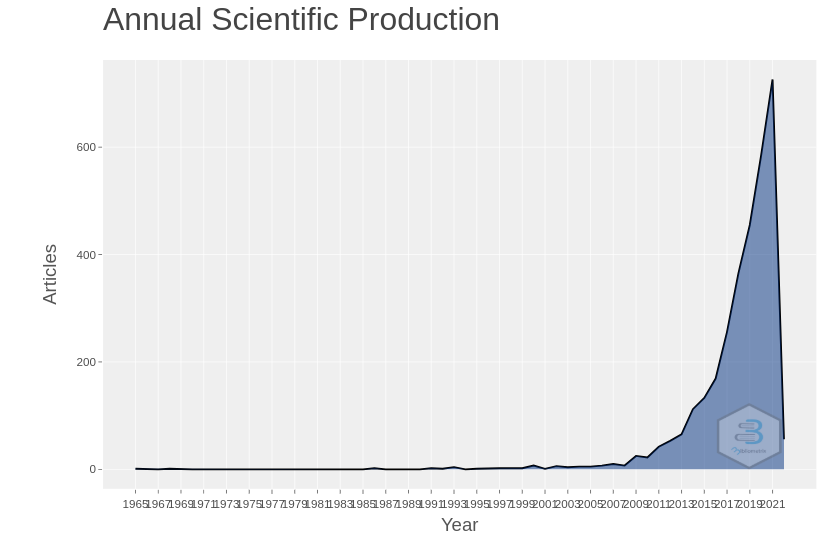
\includegraphics[width=1\textwidth]{experiments/GustavoMacCar/AnaliseBibliometrica/PsychDiseasesTech/anual-scientific-production.png}
    \caption{Evolução da produção científica no \dataset\ ao longo do tempo.}
    \label{fig:evol:anual:psych}
\end{figure}

A figura \ref{fig:evol:anual:psych} apresenta como a produção científica a respeito do tema deste estudo foi variando ao longo do tempo.

O \textit{Annual Growth Rate} do \dataset\   é de 12,19\% .

\subsection{Interpretação do Crescimento} Podemos perceber pela figura \ref{fig:evol:anual:psych} que o tema teve uma produção irrisória dentre os anos de 1965 até meados do início da década de 2000. Isso pode sugerir
que alguns registros incluídos na \texttt{query} não abordam o tema deste estudo de forma adequada, tendo em vista que os objetos tecnológicos abordados por este estudo só vieram a se popularizar pela década de 2010. A partir do
ano de 2011, pôde-se observar um aumento acentuado na produção científica a respeito desse tema e, ao longo do tempo, esse aumento foi se intensificando ainda mais. Isso sugere que, assim que a tecnologia começou a se popularizar, surgiu também
a preocupação a respeito da correlação entre a tecnologia e as enfermidades psiquiátricas abordadas nessa pesquisa e essa preocupação foi aumentando juntamente com o avanço da tecnologia. Pelo fato deste estudo ter sido conduzido em fevereiro de 2022,
não é possível afirmar que a pequena quantidade de artigos publicados após 2021 no \dataset\ representa uma queda no interesse pelo tema.
\subsection{Evolução das Citações}

\begin{figure}
    \centering
    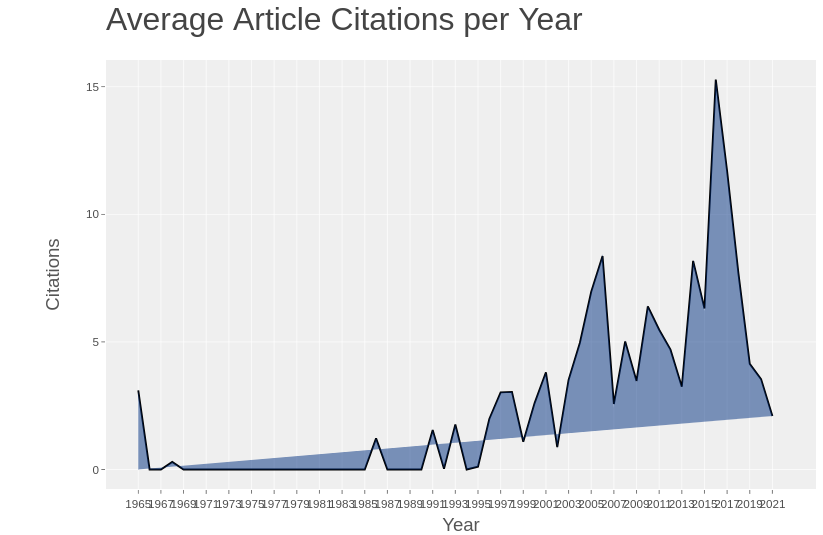
\includegraphics[width=1\textwidth]{experiments/GustavoMacCar/AnaliseBibliometrica/PsychDiseasesTech/citations-per-year.png}
    \caption{Evolução das citações aos artigos presentes no \dataset\ .}
    \label{fig:evol:anual:citations:psych}
\end{figure}

A figura \ref{fig:evol:anual:citations:psych} apresenta como as citações aos artigos no \dataset\ evoluíram ao longo do tempo. 
Nota-se uma grande variação ao longo dos anos na média de citações.

\subsection{Interpretação das Citações}
A grande variação na quantidade média de citações pode sugerir que o tema se torna mais relevante em determinados períodos ou então que algum artigo tenha sido citado várias vezes em um determinado ano. 
Uma evidência que apoia essa segunda hipótese é que ao ignorarmos os anos em que houve um pico na média de citações, podemos notar um aumento mais estável, o que é compatível com o aumento na quantidade de artigos publicados.

\subsection{\textit{Three-Field Plots (Sankey diagram)}}


\begin{figure}
    \centering
    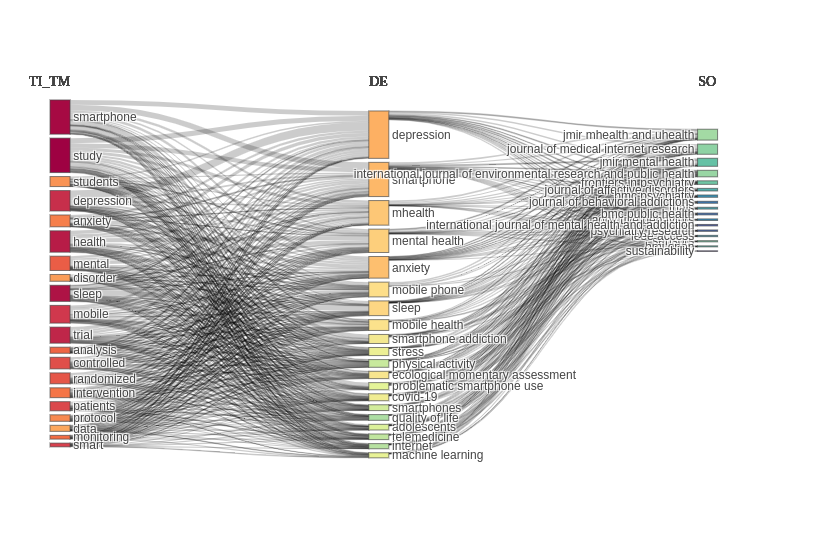
\includegraphics[angle=0,width=1\textwidth]{experiments/GustavoMacCar/AnaliseBibliometrica/PsychDiseasesTech/sankey.png}
    \caption{Plotagem ``Três Campos'' (Sankey plot) do \dataset\ . 20 Títulos, Palavras-Chave e fontes mais proeminentes, respectivamente.}
    \label{fig:sankey:psych}
\end{figure}

A figura \ref{fig:sankey:psych} apresenta a plotagem do tipo ``Três Campos'' do \dataset\. Estão representados títulos na coluna da esquerda, palavras-chave na coluna do meio e fontes na coluna da direita. Foram escolhidos 20 valores para cada coluna.

\subsection{Interpretação da figura \ref{fig:sankey:psych}}
Ao avaliarmos os títulos na coluna da esquerda, podemos inferir que os \texttt{smartphones} são os dispositivos tecnológicos mais relacionado aos problemas psiquiátricos citados. A julgar pelas fontes na coluna da direita, podemos inferir que as comunidades que mais 
estudam a correlação entre tecnologia e depressão, ansiedade e insônia é a comunidade médica, com destaque para os estudos sobre saúde mental. A enfermidade com maior destaque parece ser a depressão.

\subsection{Palavras mais frequentes}

Ao analisarmos as 50 palavras mais frequentes no \dataset, não é possível identificar nenhuma palavra sugestiva de um artigo fora do tema da pesquisa. Assim sendo, apesar de retornar registros de uma época em que os dispositivos tecnológicos em consideração não existiam e, portanto,
não abordam o tema deste estudo, tais registros foram encontrados em quantidades muito pequenas e insuficientes para viesar os resultados.

\begin{figure}[htp]
    \centering
    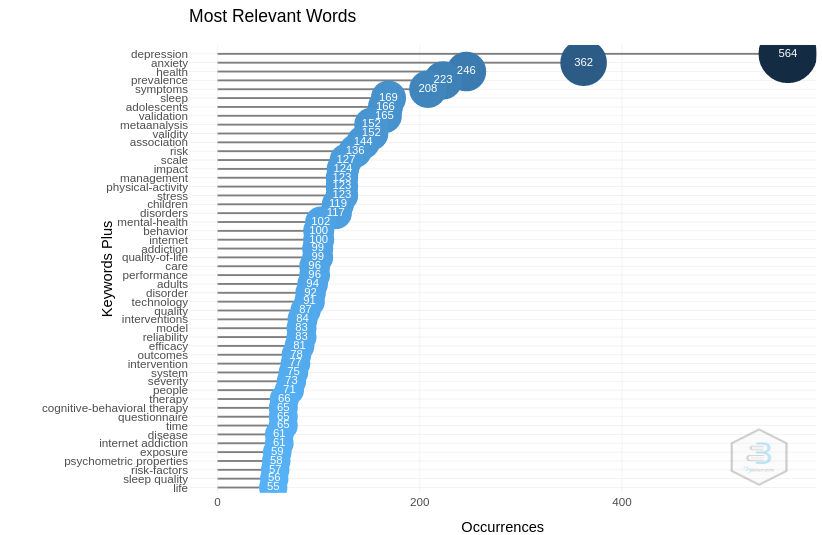
\includegraphics[angle=0,width=1\textwidth]{experiments/GustavoMacCar/AnaliseBibliometrica/PsychDiseasesTech/mfw.png}
    \caption{50 palavras mais frequentes no \dataset\ .}
    \label{fig:psych:mfw}
\end{figure}